% !TeX encoding = UTF-8

\documentclass[11pt]{amsart}

\usepackage{tikz,
pgfplots,
graphicx,
caption,
subcaption,
tikzscale,
multirow,
appendix,
pgfplotstable,
cite,
hyperref
}
\usepackage[margin=0.7in]{geometry}
\usetikzlibrary{plotmarks}
\usepgfplotslibrary{groupplots}

\colorlet{linecolora}{blue}
\colorlet{linecolorb}{red}
\colorlet{linecolorc}{brown}
\colorlet{linecolord}{black}

\newcommand{\markOne}{*}
\newcommand{\markTwo}{triangle*}
\newcommand{\markThree}{square*}
\newcommand{\markFour}{diamond*}


\newcommand{\tikzPlotStylea}{

\begin{tikzpicture}
\draw[linecolora] plot[mark = \markOne] (0,0);
\end{tikzpicture}
}

\newcommand{\tikzPlotStyleb}{
\begin{tikzpicture}
\draw [linecolorb] plot[mark = \markTwo] (0,0);
\end{tikzpicture}
}

\newcommand{\tikzPlotStylec}{

\begin{tikzpicture}
\draw [linecolorc] plot[mark = \markThree] (0,0);
\end{tikzpicture}
}

\newcommand{\tikzPlotStyled}{

\begin{tikzpicture}
\draw [linecolord] plot[mark = \markFour] (0,0);
\end{tikzpicture}
}

\pgfplotsset{
plotoptsa/.style={only marks,color=linecolora,mark=\markOne},
plotoptsb/.style={only marks,color=linecolorb,mark=\markTwo},
plotoptsc/.style={only marks,color=linecolorc,mark=\markThree},
plotoptsd/.style={only marks,color=linecolord,mark=\markFour}
}


\newcommand{\addGroupPlotToFigure}[2]{
\addplot+[
		  plotoptsa,
          error bars/.cd,
		  y explicit, y dir=both,
		]
table[linecolora,x =x,y =y,y error =yp,col sep = comma]{#1-small-small-subplot-#2};
\addplot+[
		  plotoptsb,
          error bars/.cd,
		  y explicit, y dir=both,
		]
table[linecolorb,x =x,y =y,y error =yp,col sep = comma]{#1-small-big-subplot-#2};
\addplot+[
		  plotoptsc,
          error bars/.cd,
		  y explicit, y dir=both,
		]
table[linecolorc,x =x,y =y,y error =yp,col sep = comma]{#1-big-small-subplot-#2};
\addplot+[
 		  plotoptsd,
          error bars/.cd,
		  y explicit, y dir=both,
		]
table[linecolord,x =x,y =y,y error =yp,col sep = comma]{#1-big-big-subplot-#2};
}

\newcommand{\addGhostGroupPlotToFigure}[2]{
\addplot+[
		  draw = none,
		]
table[draw = none,mark =none, x =x,y expr = {\thisrow{y}+\thisrow{yp}},col sep = comma]{#1-small-small-subplot-#2};
\addplot+[
          draw = none,
		]
table[draw = none,mark =none, x =x,y expr = {\thisrow{y}+\thisrow{yp}},col sep = comma]{#1-small-big-subplot-#2};
\addplot+[
          draw = none,
		]
table[draw = none,mark =none, x =x,y expr = {\thisrow{y}+\thisrow{yp}},col sep = comma]{#1-big-small-subplot-#2};
\addplot+[
          draw = none,
		]
table[draw = none,mark =none, x =x,y expr = {\thisrow{y}+\thisrow{yp}},col sep = comma]{#1-big-big-subplot-#2};
\addplot+[
		  draw = none,
		]
table[draw = none,mark =none, x =x,y expr = {\thisrow{y}-\thisrow{ym}},col sep = comma]{#1-small-small-subplot-#2};
\addplot+[
          draw = none,
		]
table[draw = none,mark =none, x =x,y expr = {\thisrow{y}-\thisrow{ym}},col sep = comma]{#1-small-big-subplot-#2};
\addplot+[
          draw = none,
		]
table[draw = none,mark =none, x =x,y expr = {\thisrow{y}-\thisrow{ym}},col sep = comma]{#1-big-small-subplot-#2};
\addplot+[
          draw = none,
		]
table[draw = none, mark =none, x =x,y expr = {\thisrow{y}-\thisrow{ym}},col sep = comma]{#1-big-big-subplot-#2};
}
\newcommand{\makeFigureAllSizes}[2]{
\pgfplotstableread{#1-small-small-subplot-1}\tableA
\pgfplotstableread{#1-small-small-subplot-2}\tableB
\pgfplotstableread{#1-small-small-subplot-3}\tableC
\pgfplotstableread{#1-small-small-subplot-4}\tableD
\pgfplotssetlayers
\begin{tikzpicture}
\begin{groupplot}[group style = {group size =2 by 2,
			group name = the plots,
			xlabels at = edge bottom,
			ylabels at = edge left
                                },
			width = .4\linewidth,
			height = .3\linewidth,
			scale only axis = true,		    
   			xlabel = {Fraction Consumers as parasites},
			ylabel = {#2},
			x label style = {font=\tiny},
			y label style = {font=\tiny},
		    legend style={ ,at={(-.15,-.23)},
						   anchor=north,
						   font=\tiny},
			legend columns = 4,
			grid = both,
			unbounded coords = jump,
			%ymin = 0,ymax = 1,
]
\nextgroupplot[xticklabels={}]
\addGroupPlotToFigure{#1}{1}
\addGhostGroupPlotToFigure{#1}{2}
\addGhostGroupPlotToFigure{#1}{3}
\addGhostGroupPlotToFigure{#1}{4}
\nextgroupplot[xticklabels={},yticklabels={}]
\addGroupPlotToFigure{#1}{2}
\addGhostGroupPlotToFigure{#1}{1}
\addGhostGroupPlotToFigure{#1}{3}
\addGhostGroupPlotToFigure{#1}{4}
\nextgroupplot
\addGroupPlotToFigure{#1}{3}
\addGhostGroupPlotToFigure{#1}{2}
\addGhostGroupPlotToFigure{#1}{1}
\addGhostGroupPlotToFigure{#1}{4}
\nextgroupplot[yticklabels={}]
\addGroupPlotToFigure{#1}{4}
\addGhostGroupPlotToFigure{#1}{2}
\addGhostGroupPlotToFigure{#1}{3}
\addGhostGroupPlotToFigure{#1}{1}
\legend{$Z_f=10;Z_p = 10^{-3}$,
$Z_f=10;Z_p = 10^{-4}$,
$Z_f=100;Z_p = 10^{-3}$,
$Z_f=100;Z_p = 10^{-4}$}
\end{groupplot}
\node [text width =.5\linewidth,align=center,anchor=south] at (the plots c1r1.north) {\subcaption[]{ Null model\label{fig:#1-a}}};
\node [text width =.5\linewidth,align=center,anchor=south] at (the plots c2r1.north) {\subcaption[]{Refuge\label{fig:#1-b}}};
\node [text width =.5\linewidth,align=center,anchor=south] at (the plots c1r2.north) {\subcaption[]{Concomittant \label{fig:#1-c}}};
\node [text width =.5\linewidth,align=center,anchor=south] at (the plots c2r2.north) {\subcaption[]{Refuge with Concomittant\label{fig:#1-d}}};
\begin{pgfonlayer}{axis background}
\node [opacity = 0.4,] at (the plots c1r1.center) {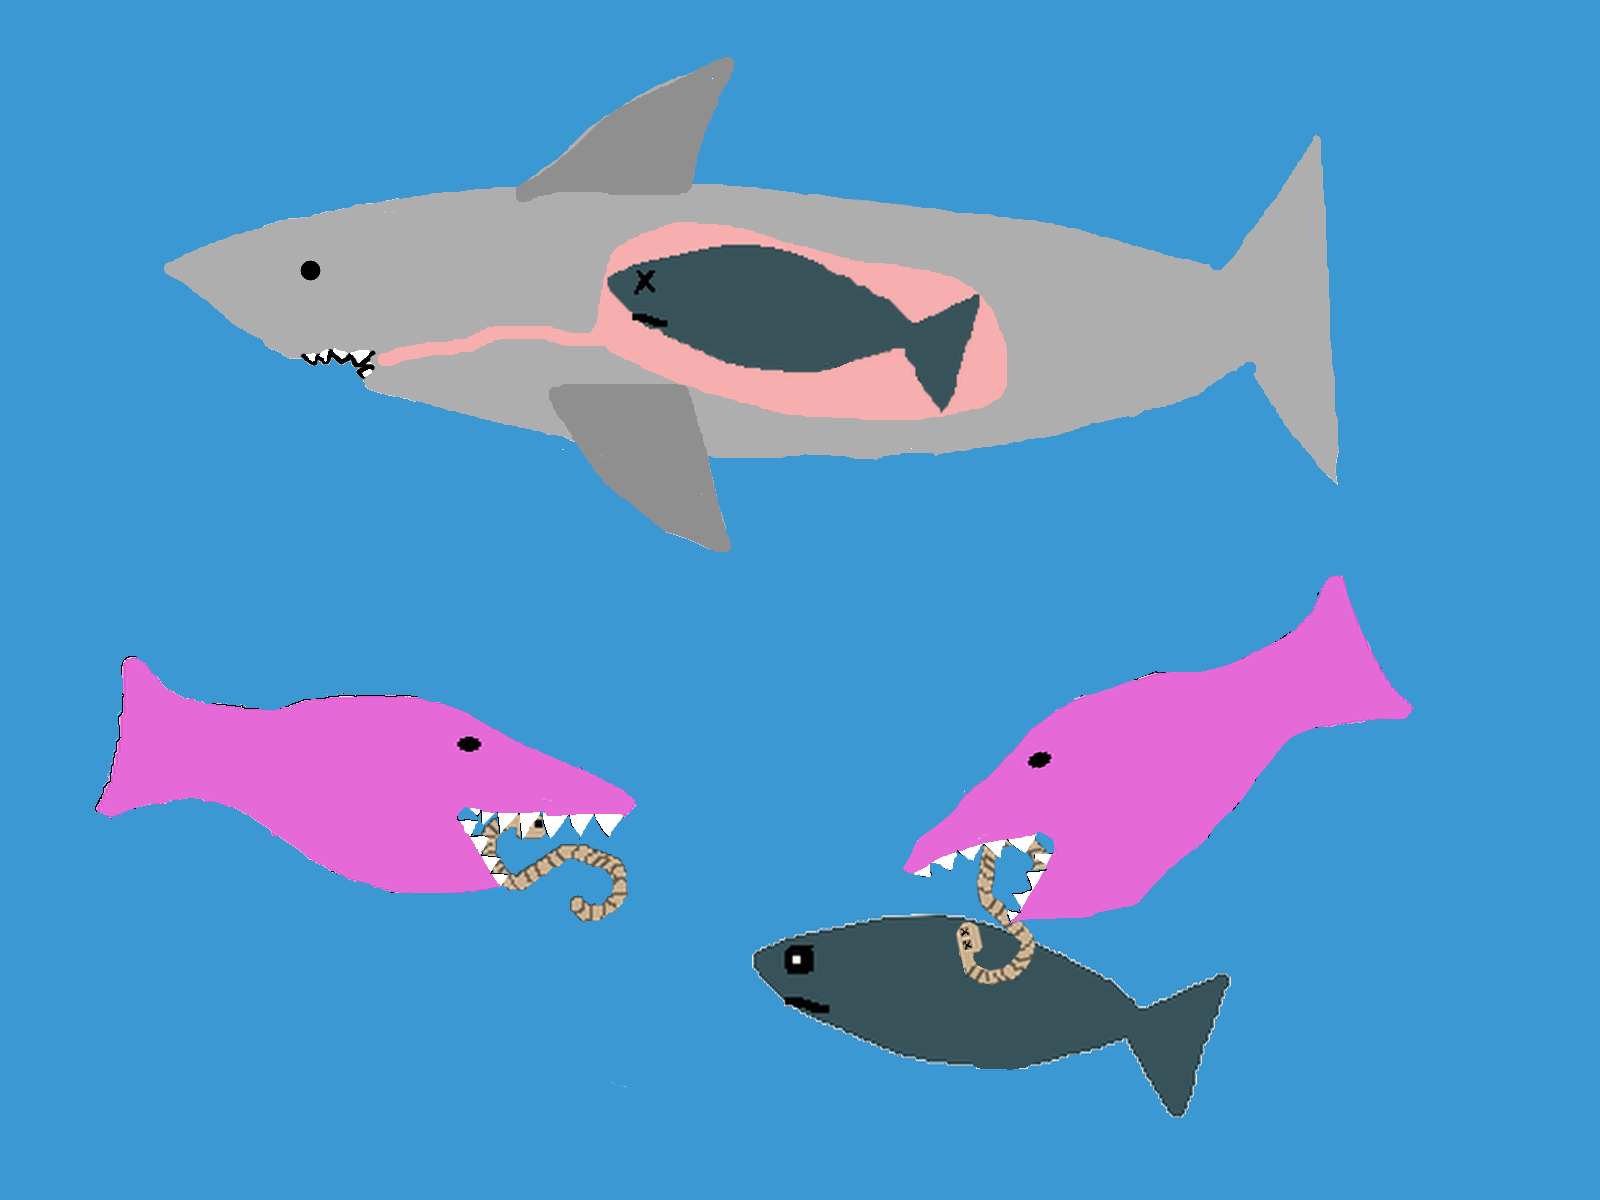
\includegraphics[width=.4\linewidth]{../../figures/Null.png}};
\node [opacity = 0.4,] at (the plots c2r1.center) {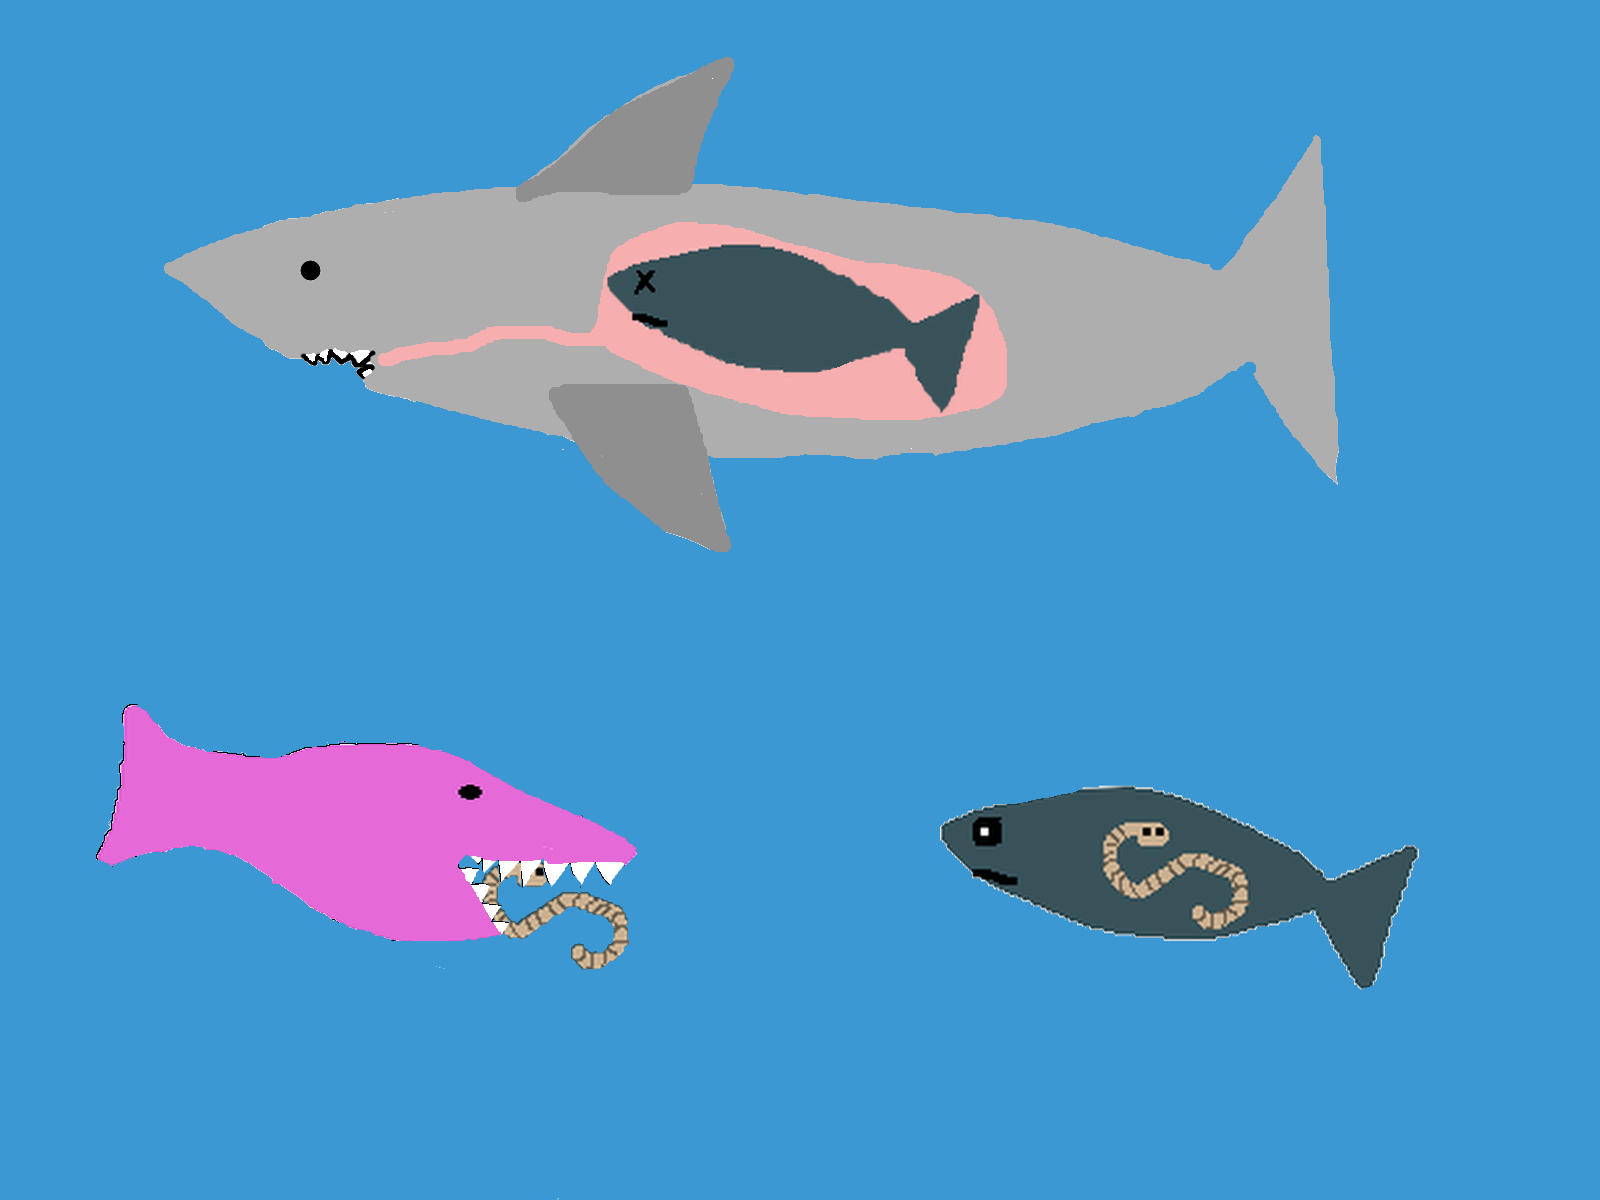
\includegraphics[width=.4\linewidth]{../../figures/Null+Ref.png}};
\node [opacity = 0.4,] at (the plots c1r2.center) {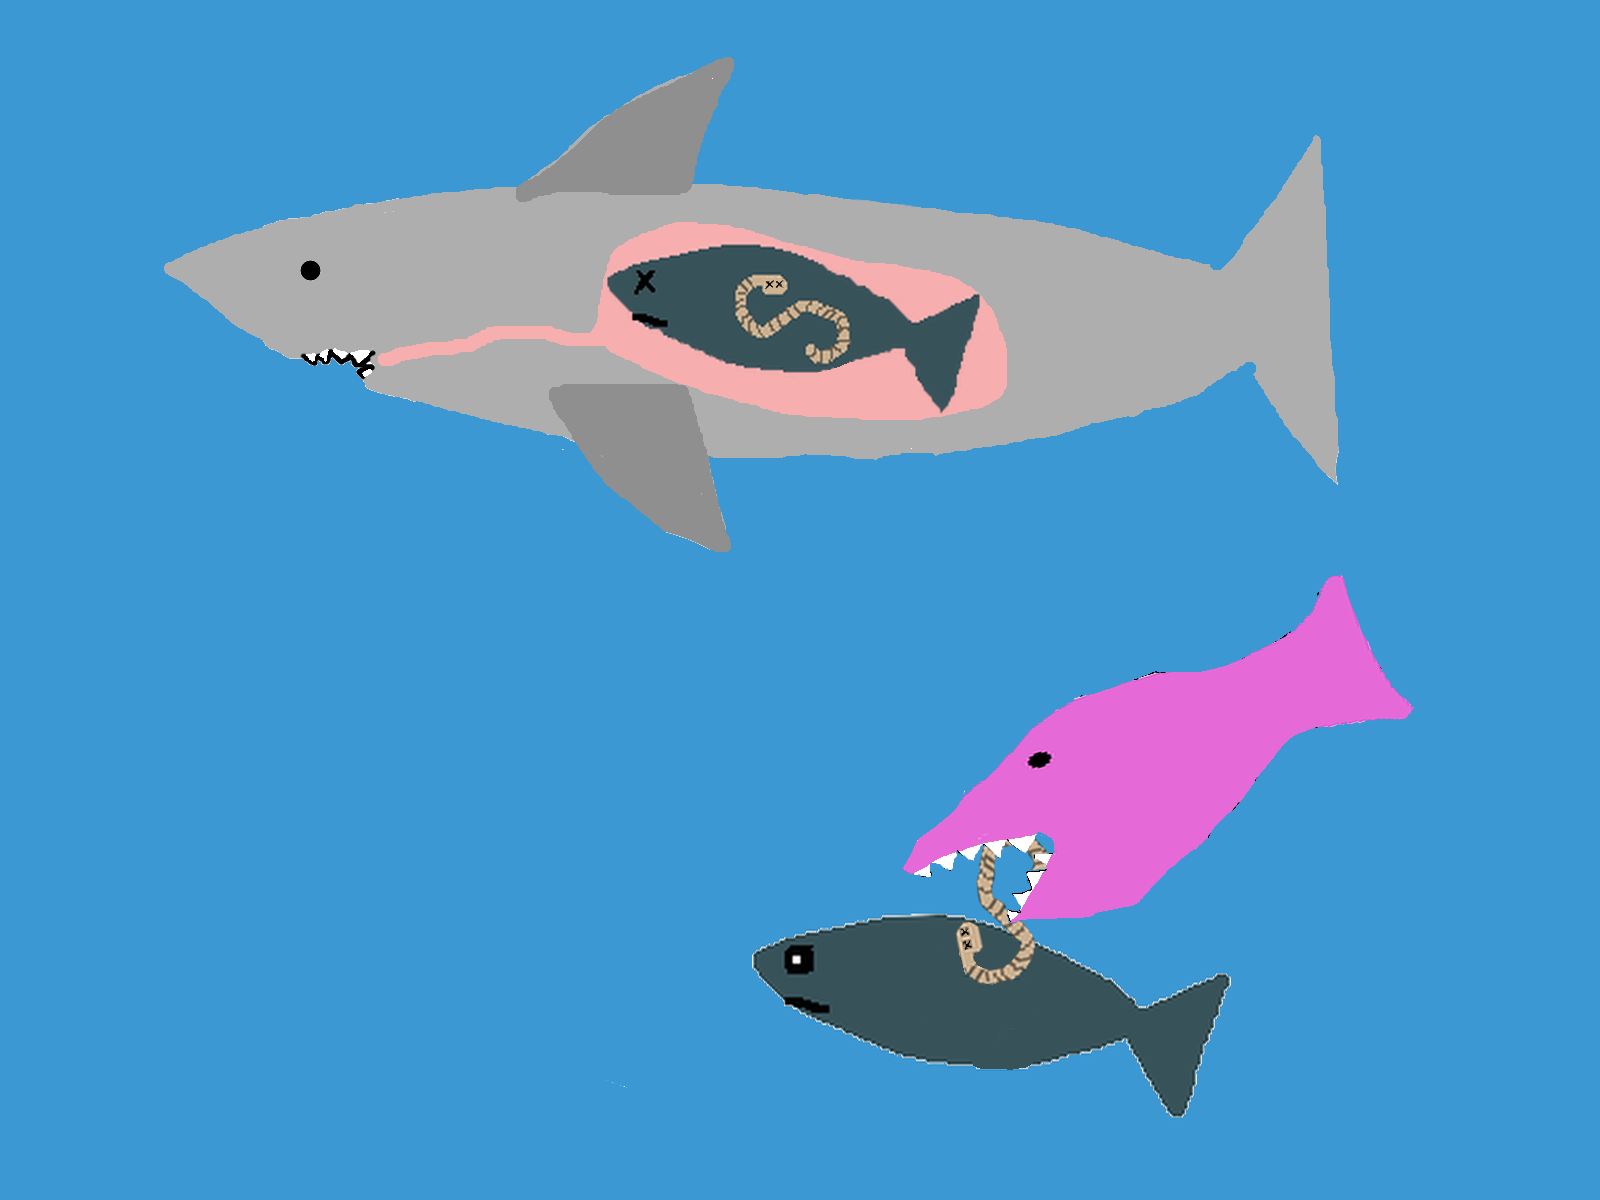
\includegraphics[width=.4\linewidth]{../../figures/Null+Con.png}};
\node [opacity = 0.4,] at (the plots c2r2.center) {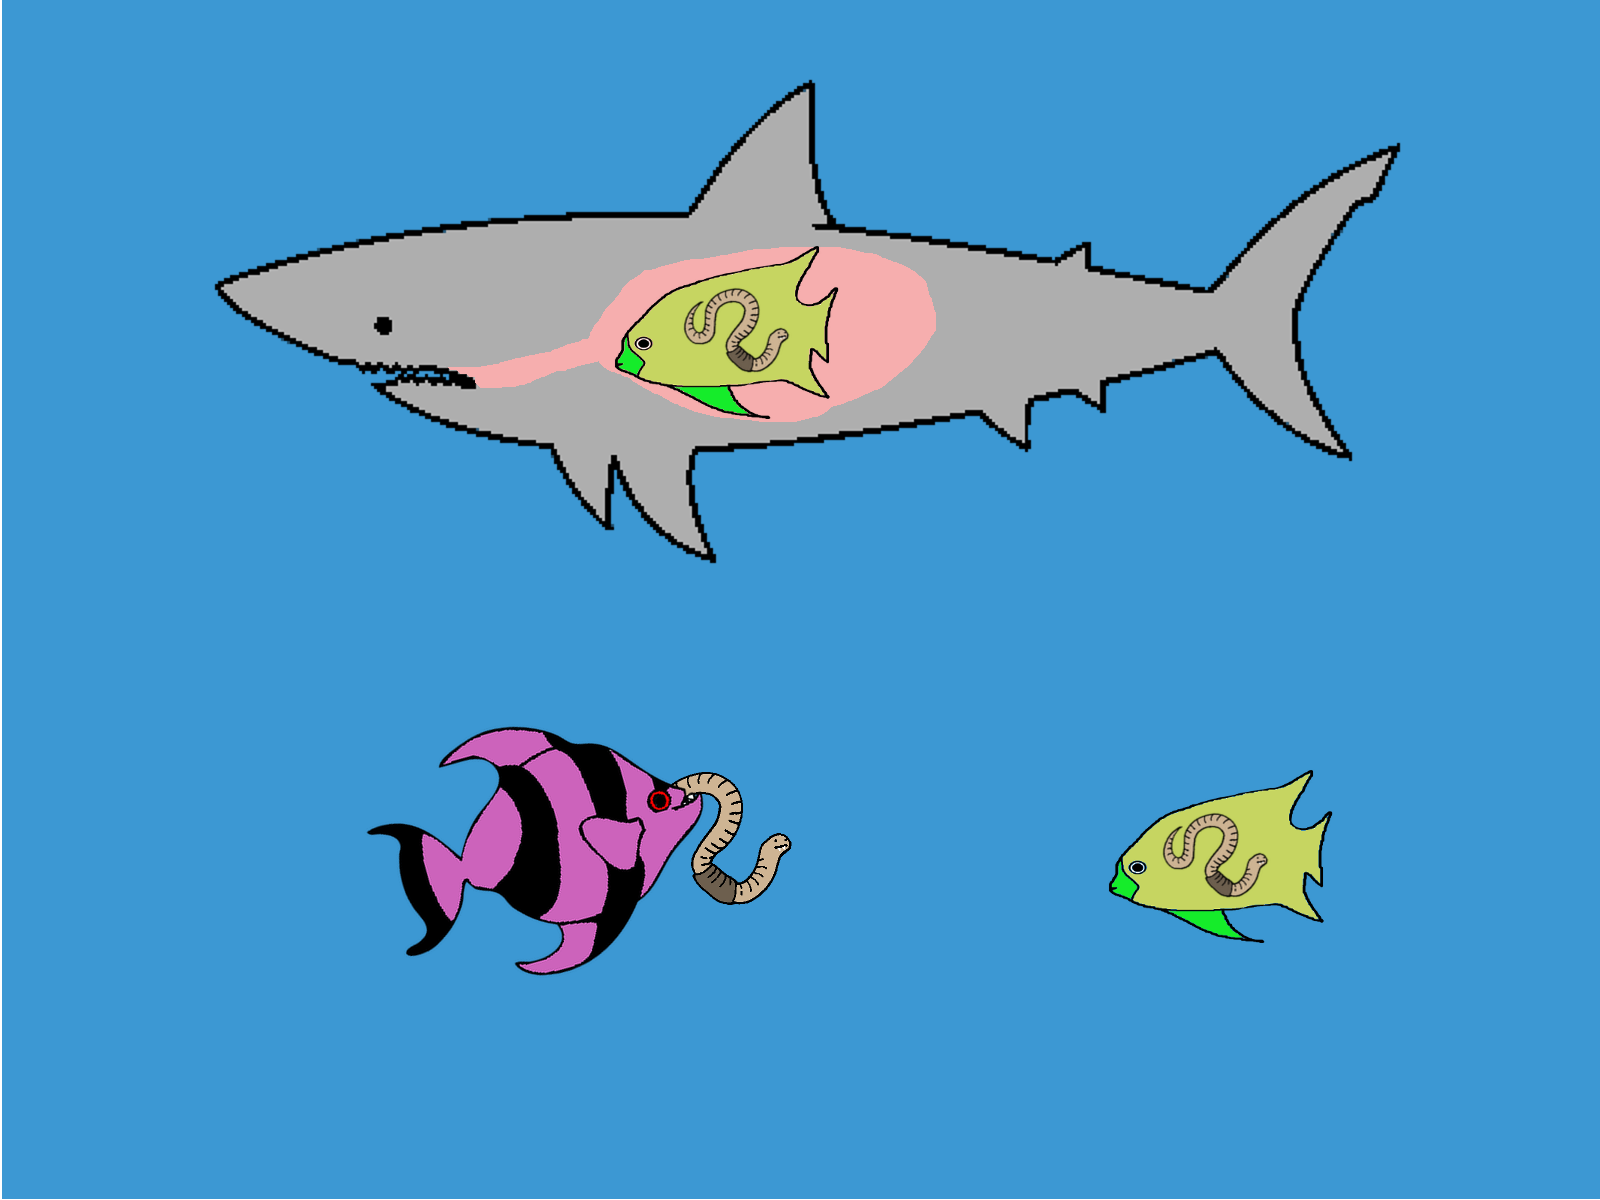
\includegraphics[width=.4\linewidth]{../../figures/Con+Ref.png}};
\end{pgfonlayer}
\end{tikzpicture}
}

\newcommand{\makeFigureAllModels}[2]{
\begin{tikzpicture}
\begin{axis}[
		    xlabel = {Fraction Consumers as parasites},
			ylabel = {#2},
		    legend style={ ,at={(-.45,-.33)},
						   ,anchor=south},
			legend columns = 2,
]

\addplot+[
		  only marks, mark = o,
          error bars/.cd,
		  y explicit, y dir=both,
		]
table[blue, x =x,y =y,y error =yp,col sep = comma]{#1-1};
\addplot+[
		  only marks, mark = triangle,
          error bars/.cd,
		  y explicit, y dir=both,
		]
table[red,x =x,y =y,y error =yp,col sep = comma]{#1-2};
\addplot+[
		  only marks, mark = square,
          error bars/.cd,
		  y explicit, y dir=both,
		]
table[brown,x =x,y =y,y error =yp,col sep = comma]{#1-3};
\addplot+[
		  only marks, mark = diamond,
          error bars/.cd,
		  y explicit, y dir=both,
		]
table[black,x =x,y =y,y error =yp,col sep = comma]{#1-4};
\legend{Null Model,
 Host Refuge,
 Concomittant Only,
 Refuge with Concomittant}
\end{axis}
\end{tikzpicture}
}


\pgfplotsset{table/search path={../data/},compat=newest}
\title{Results}
\author{Nick}


\begin{document}
\section{Persistence of Final States}


\begin{figure}[h] 
\captionsetup[subfigure]{labelfont = it, textfont = it,labelformat = parens,labelsep = space}
    \begin{minipage}{.45\textwidth}
        \phantomsubcaption{\label{fig:persistence-a}}
    \end{minipage}
    \begin{minipage}{.45\textwidth}
        \phantomsubcaption{\label{fig:persistence-b}}
    \end{minipage}
    \includegraphics[width=\textwidth]{../floats/results/perAll.png}
        \caption{The figure shows the total persistence with 95\% confidence intervals of all species in all models with all body size configurations.  Differences plots and fix scales.}
    \begin{minipage}{.45\textwidth}
        \phantomsubcaption{\label{fig:persistence-c}}
    \end{minipage}
    \begin{minipage}{.45\textwidth}
        \phantomsubcaption{\label{fig:persistence-d}}
    \end{minipage}
\label{fig:persistenceAll}
\end{figure}

Figure \ref{fig:persistenceAll} shows the average persistence of the web ensemble with different body size ratios and the different dynamical models.\footnote{Think about what a null hypothesis might be in this setting: show what the line is if all parasites go extinct?  If free livers maintain the same extinction level?  Is that encessary..}  Adding more parasites clearly results in a decrease in the overall persistence of the web.  This should not be terribly surprising since we have seen that low body size ratios are associated with lower overall persistence in food webs.  Note that the result shown here is slightly different\footnote{look up the numbers from Brose 2006; compare those results with the average body size ratio in each model.  Also compare average body size ratios within my models.  Would also be useful to compare the free-living and parasitic subsets (and their average body size ratios) with the Brose results, for more direct connection to previous work.  Beware: published results have drawbacks (low extinction threshold with short simulation time means species don't have enough time to go extinct).} since only certain fractions of consumers are subjected to the inverted body size ratios. It could be partially explained by parasites going extinct at disproportionately higher levels.  This is true to some extent, but it is not the whole story (see figures \ref{fig:persistenceFree} and \ref{fig:persistencePara} in sections \ref{sec:persistenceFree} and \ref{sec:persistencePara}, respectively).

When there are no parasites in the null model (figure \ref{fig:persistence-a}), the average persistence of food webs with a consumer-resource body size ratio (BSR) of 10 is higher than of food webs with a consumer-resource BSR of 100.  This pattern reverses at higher levels of parasitism.  We can infer from this that food webs with an underlying free-living BSR of 100 are more resilient to additions of parasites.  The mechanism for this resilience is not explained by this study.\ref{fig:persistenceAll}\footnote{Maybe if I dig into the time series;  Species with low metabolic rates can 'outlast' high pressure from the parasites? Parasites themselves are larger and have lower absolute metabolic rats? Something more complicated?  Maybe after all the extinctions we get two sort of parallel structures, one of mostly free-livers and one of mostly parasites?  It probably has a lot to do with the amount of energy extracted from basal species; the interface of the changing $x_i$ with the static $r_i$.}   Another general pattern we observe is that adding parasites with a parasite-host BSR of $1/1,000$ is less detrimental to stability than adding parasites with a parasite-host BSR of $1/10,000$.  That is, if the consumer-resource BSR of free livers is held constant, webs with a parasite-host BSR of $1/10,000$ are less persistent than webs that have a parasite-host BSR of $1/1,000$.

The interaction of both patterns means that at the highest parasite levels, the most resilient consumer-resource BSR and the least disruptive parasite-host BSR (brown data series) resulted in a relative decrease in persistence of only about 16\% (from 58\% persistence to 49\% persistence).  The more resilient consumer-resource BSR paired with the more disruptive parsite-host BSR (black data series) had a relative loss in persistence of about 22\% (from 58\% to 45\% persistence). The less resilient consumer-resource BSR paired with the less disruptive parasite-host BSR (blue data series) had the same level of persistence as the black data series, but this corresponded to a relative decrease of about 32\% (from 66\% to 45\% persistence).  Finally, the least resilient consumer-resource BSR paired with the more disruptive parasite-host BSR had the lowest average persistence and the highest relative decrease of 45\% (from 66\% to 38\% persistence). 

It should of course be noted that when parasites comprise 50\% of all consumers, there is quite a bit of 'cross-pollination' of links.  That is, there are quite a few links between two parasites (for which the average BSR is the same as for free livers) or links with a free living consumer and parasitic prey (for which the average BSR is much higher than the average BSR for free livers).  This effect is less pronounced\footnote{Try to get some numbers to quantify it} at lower parasite levels.  Regardless, in the empirical data we only see abut 20-30\% of consumers as parasites.  For these ranges, the brown, blue, and black data series all have very similar persistence levels (though this is true at higher levels as well) and the red data series is close at 20\% parasitism and more noticeably lower at 30\% parasitism.

Another interesting feature of these data is that (at 50\% parasitism) the data series with the highest persistence also has the highest average consumber-resource BSR.\footnote{Need to get the exact number; not quite as simple as averaging the two but I think it's a good approximation at this point.}  The two data series with the next lowest persistence level have a lower average BSR; they also have approximately the same persistence and approximately the same average BSR.  The red data series has the lowest average body size ratio and the lowest persistence level.  This is intriguingly similar to the results from \cite{Brose2006}.\footnote{A good thing to look at might be the change in body size ratio distributions before and after extinctions for different initial body size ratios - hasn't that been done..?} 
Adding Concomittant predation to the null model (figure \ref{fig:persistence-c}) had little qualitative effect on the persistence patterns.  Quantitatively, concomittant predation results in a slightly lower average persistence level, though this is qutie hard to make out in the graphs and seems to be a very small effect.\footnote{Need to quantify this as well.  Average difference in persistence maybe - could do it as a plot?}

Splitting the parasitic biomass into a fraction inside and and a fraction outside of their hosts (figure \ref{fig:persistence-b}) initially (in terms of increasing parasite fraction) causes a faster decrease in persistence.  
Furthermore, the persistence does not level out as in the other two models (left column) but continues decreasing up to the highest level of parsitism.  Adding concomittant predation to this model (figure \ref{fig:persistence-d}) again had little discernable effect on the average persistence.

\subsection{Free Living Consumer Persistence \label{sec:persistenceFree}}

The results for free liver persistence are almost identical to the results for the persistence of all species (figure \ref{fig:persistenceAll}); the patterns are basically the same, but the actual persistence at a given parasite level is a few percentage points lower.  This isn't surprising, since the overall persistence takes into account basal species, which never go extinct in the model.  That discrepancy is not the only difference, however.

In the null model (figure \ref{fig:free-persistence-a}) the most striking difference is in the red data series, which is about 10 percentage points lower at the highest parasitism level for free livers than for all species.  This tells us that free-livers are disproportionately affected by parasites in that combination of consumer-resource and parasite-host BSR.  The story is basically the same when concomittant predation is added (figure \ref{fig:free-persistence-c}), but there does seem to be a slightly visible increase in free-living persistence\footnote{Probably not worth saying since I don't think I can really back this up}.   

When parasites are split into fractions inside and outside of their hosts (figure (\ref{fig:free-persistence-b}), the results again follow the same general pattern as in figure \ref{fig:persistenceAll}.  The only deviation is that both data series with a consumer-resource BSR of 10 experience a steeper decline in persistence with increasing fractions of parasites.  At the 50\% parasite level, free livers only have 20\% persistence in these webs, again about 10 percentage points lower than the persistence of all species. This is in contrast to the webs with a consumer-resource BSR of 100, which are only about 3 points lower than the total persistence result.  That is about the decrease we would expect to see just from changing our accounting from all species to free livers, since that is about the decrease in the case with no parasites.  Adding concomittant predation to the model with parasitic life stages (figure \ref{fig:free-persistence-d}) does very little to this pattern. 

\begin{figure}[h] 
\captionsetup[subfigure]{labelfont = it, textfont = it,labelformat = parens,labelsep = space}
    \begin{minipage}{.45\textwidth}
        \phantomsubcaption{\label{fig:free-persistence-a}}
    \end{minipage}
    \begin{minipage}{.45\textwidth}
        \phantomsubcaption{\label{fig:free-persistence-b}}
    \end{minipage}
    \includegraphics[width=\textwidth]{../floats/results/perFree.png}
\caption{The figure shows the total persistence with 95\% confidence intervals of free livers in all models with all body size configurations.}
    \begin{minipage}{.45\textwidth}
        \phantomsubcaption{\label{fig:free-persistence-c}}
    \end{minipage}
    \begin{minipage}{.45\textwidth}
        \phantomsubcaption{\label{fig:free-persistence-d}}
    \end{minipage}
\label{fig:persistenceFree}
\end{figure}

\subsection{Parasitic Consumer Persistence \label{sec:persistencePara}}

The persistence of parasites in these models follows strikingly different patterns than the persistence of free livers (figure \ref{fig:persistencePara}).  In the null model (figure \ref{fig:para-persistence-a}), the blue data series (that is, more susceptible free livers and less disruptive parasites) clearly has the highest persistence at low levels of parasitism and stays roughly constant throughout all levels of parasitism\footnote{would be great to have a regression equation here.}.  The red data series (more susceptible free livers and more disruptive parasites) also stays roughly the same over all levels of parsitism.   By contrast, the brown and black data series have very low persistence levels at 5\% parasites, then increase to nearly double their original persistence at 50\% parasites.

Adding concomittant losses (figure \ref{fig:para-persistence-c}) doesn't change the overall pattern of persistence, but as before, does decrease the overall parasitic persistence at every parasite level by as much as 10 percentage points.  The black and brown data series show the same increasing trend as in figure \ref{fig:para-persistence-a}, but again the mean values are about 3-5 percentage points lower.a

Adding a refuge for a fixed percentage of parasitic biomass (figure \ref{fig:para-persistence-b}) dramatically changes the pattern of parasitic persistence.  At low levels of parasitism, the persistence approximately matches that in figure \ref{fig:para-persistence-a}, but as the percentage of parasites increases, we see the red and blue data series start to decrease, where before they were constant.  In this case the brown and the black data series maintain very low levels of persistence (about 10\%) for all levels of parasitism.\footnote{This looks like the effect could be explained by a roughly linear (in parasite percentage) decrease in persistence.  This would be cool to work out, but maybe not of much value.}

  Adding concomittant predation (figure \ref{fig:para-persistence-d}) doesn't change the qualitative behavior but each data series is once again shifted down by a few percentage points.  Average persistence never really drops below about 8\%, so the brown and black data series only saw a drop of 2-3\%, while the blue data series experienced a drop of about 10\% in average persistence at low parasite levels.  At high levels of parasitism all four combinations of parasite and free liver body sizes have persistence in the 10-12\% range.

\begin{figure}[h]
\captionsetup[subfigure]{labelfont = it, textfont = it,labelformat = parens,labelsep = space}
    \begin{minipage}{.45\textwidth}
        \phantomsubcaption{\label{fig:para-persistence-a}}
    \end{minipage}
    \begin{minipage}{.45\textwidth}
        \phantomsubcaption{\label{fig:para-persistence-b}}
    \end{minipage}
    \includegraphics[width=\textwidth]{../floats/results/perPara.png}
\caption{The figure shows the total persistence with 95\% confidence intervals of free livers in all models with all body size configurations.}
    \begin{minipage}{.45\textwidth}
        \phantomsubcaption{\label{fig:para-persistence-c}}
    \end{minipage}
    \begin{minipage}{.45\textwidth}
        \phantomsubcaption{\label{fig:para-persistence-d}}
    \end{minipage}
\caption{The figure shows the persistence of parasites with 95\% confidence intervals in all models with all body size configurations.}
\label{fig:persistencePara}
\end{figure}


\subsection{Order of extinctions\label{sec:extinctionOrders}}

\begin{figure}[h]
\captionsetup[subfigure]{labelfont = it, textfont = it,labelformat = parens,labelsep = space}
    \begin{minipage}{.45\textwidth}
        \phantomsubcaption{\label{fig:pred-persistence-a}}
    \end{minipage}
    \begin{minipage}{.45\textwidth}
        \phantomsubcaption{\label{fig:pred-persistence-b}}
    \end{minipage}
    \includegraphics[width=\textwidth]{../floats/results/preyFirst.png}
\caption{The figure shows the total persistence with 95\% confidence intervals of free livers in all models with all body size configurations.}
    \begin{minipage}{.45\textwidth}
        \phantomsubcaption{\label{fig:pred-persistence-c}}
    \end{minipage}
    \begin{minipage}{.45\textwidth}
        \phantomsubcaption{\label{fig:pred-persistence-d}}
    \end{minipage}
\caption{This figure shows the average fraction of a species' prey that go extinct first with 95\% confidence intervals in all models with all body size configurations. \label{fig:frac-prey-first}}
\end{figure}
%TODO explain the calculation better
The order of extinctions in food webs in general is an under-studied question (but see the NU people).  In this section we attempt to understand how the fraction of parasites in food webs affects the order of extinctions in ATN models.  Figure \ref{fig:frac-prey-first} shows the average (over all webs) of the average (over all species in a web) fraction of prey items that go extinct before each species\footnote{Surprisingly difficult to caculate/ambiguous since I had to make quite a few choices here.}.  Here we see a striking differene between the more resilient free-livers and the less resilient free lievers.  The simulations with more resilient free-livers tended to see about half a species diet go extinct before
 
\begin{figure}[h]
\captionsetup[subfigure]{labelfont = it, textfont = it,labelformat = parens,labelsep = space}
    \begin{minipage}{.45\textwidth}
        \phantomsubcaption{\label{fig:prey-persistence-a}}
    \end{minipage}
    \begin{minipage}{.45\textwidth}
        \phantomsubcaption{\label{fig:prey-persistence-b}}
    \end{minipage}
    \includegraphics[width=\textwidth]{../floats/results/predFirst.png}
\caption{The figure shows the total persistence with 95\% confidence intervals of free livers in all models with all body size configurations.}
    \begin{minipage}{.45\textwidth}
        \phantomsubcaption{\label{fig:prey-persistence-c}}
    \end{minipage}
    \begin{minipage}{.45\textwidth}
        \phantomsubcaption{\label{fig:prey-persistence-d}}
    \end{minipage}
\caption{This figure shows the average fraction of a species' pred that go extinct first with 95\% confidence intervals in all models with all body size configurations.\label{fig:frac-pred-first}}
\end{figure}

\subsection{Persistence by Trophic Level}

\begin{figure}[h]
\captionsetup[subfigure]{labelfont = it, textfont = it,labelformat = parens,labelsep = space}
    \begin{minipage}{.45\textwidth}
        \phantomsubcaption{\label{fig:tl3-persistence-a}}
    \end{minipage}
    \begin{minipage}{.45\textwidth}
        \phantomsubcaption{\label{fig:tl3-persistence-b}}
    \end{minipage}
    \includegraphics[width=\textwidth]{../floats/results/perTL3.png}
    \begin{minipage}{.45\textwidth}
        \phantomsubcaption{\label{fig:tl3-persistence-c}}
    \end{minipage}
    \begin{minipage}{.45\textwidth}
        \phantomsubcaption{\label{fig:tl3-persistence-d}}
    \end{minipage}
\caption{This figure shows the persistence of all species that do not have a link directly from a basal species. \label{fig:tl3-all}}
\end{figure}

\begin{figure}[h]
\captionsetup[subfigure]{labelfont = it, textfont = it,labelformat = parens,labelsep = space}
    \begin{minipage}{.45\textwidth}
        \phantomsubcaption{\label{fig:tl3-free-persistence-a}}
    \end{minipage}
    \begin{minipage}{.45\textwidth}
        \phantomsubcaption{\label{fig:tl3-free-persistence-b}}
    \end{minipage}
    \includegraphics[width=\textwidth]{../floats/results/perTL3Free.png}
    \begin{minipage}{.45\textwidth}
        \phantomsubcaption{\label{fig:tl3-free-persistence-c}}
    \end{minipage}
    \begin{minipage}{.45\textwidth}
        \phantomsubcaption{\label{fig:tl3-free-persistence-d}}
    \end{minipage}
\caption{This figure shows the persistence of all free-living species that do not have a link directly from a basal species.\label{tl3-free}}
\end{figure}

\begin{figure}[h]
\captionsetup[subfigure]{labelfont = it, textfont = it,labelformat = parens,labelsep = space}
    \begin{minipage}{.45\textwidth}
        \phantomsubcaption{\label{fig:tl3-para-persistence-a}}
    \end{minipage}
    \begin{minipage}{.45\textwidth}
        \phantomsubcaption{\label{fig:tl3-para-persistence-b}}
    \end{minipage}
    \includegraphics[width=\textwidth]{../floats/results/perTL3Para.png}
\caption{The figure shows the total persistence with 95\% confidence intervals of free livers in all models with all body size configurations.}
    \begin{minipage}{.45\textwidth}
        \phantomsubcaption{\label{fig:tl3-para-persistence-c}}
    \end{minipage}
    \begin{minipage}{.45\textwidth}
        \phantomsubcaption{\label{fig:tl3-para-persistence-d}}
    \end{minipage}
\caption{This figure shows the persistence of all parasite species that do not have a link directly from a basal species.\label{tl3-para}}
\end{figure}

\begin{figure}[h]
\captionsetup[subfigure]{labelfont = it, textfont = it,labelformat = parens,labelsep = space}
    \begin{minipage}{.45\textwidth}
        \phantomsubcaption{\label{fig:tl2-persistence-a}}
    \end{minipage}
    \begin{minipage}{.45\textwidth}
        \phantomsubcaption{\label{fig:tl2-persistence-b}}
    \end{minipage}
    \includegraphics[width=\textwidth]{../floats/results/perTL2.png}
    \begin{minipage}{.45\textwidth}
        \phantomsubcaption{\label{fig:tl2-persistence-c}}
    \end{minipage}
    \begin{minipage}{.45\textwidth}
        \phantomsubcaption{\label{fig:tl2-persistence-d}}
    \end{minipage}
\caption{This figure shows the persistence of all species that do have a link directly from a basal species.\label{tl2-all}}
\end{figure}

\begin{figure}[h]
\captionsetup[subfigure]{labelfont = it, textfont = it,labelformat = parens,labelsep = space}
    \begin{minipage}{.45\textwidth}
        \phantomsubcaption{\label{fig:tl2-free-persistence-a}}
    \end{minipage}
    \begin{minipage}{.45\textwidth}
        \phantomsubcaption{\label{fig:tl2-free-persistence-b}}
    \end{minipage}
    \includegraphics[width=\textwidth]{../floats/results/perTL2Free.png}
    \begin{minipage}{.45\textwidth}
        \phantomsubcaption{\label{fig:tl2-free-persistence-c}}
    \end{minipage}
    \begin{minipage}{.45\textwidth}
        \phantomsubcaption{\label{fig:tl2-free-persistence-d}}
    \end{minipage}
\makeFigureAllSizes{tl2-free}{Persistence of free-living species with an autotroph prey item.}
\caption{This figure shows the persistence of free-living species that do have a link directly from a basal species.\label{tl2-free}}
\end{figure}

\begin{figure}[h]
\captionsetup[subfigure]{labelfont = it, textfont = it,labelformat = parens,labelsep = space}
    \begin{minipage}{.45\textwidth}
        \phantomsubcaption{\label{fig:tl2-para-persistence-a}}
    \end{minipage}
    \begin{minipage}{.45\textwidth}
        \phantomsubcaption{\label{fig:tl2-para-persistence-b}}
    \end{minipage}
    \includegraphics[width=\textwidth]{../floats/results/perTL2Para.png}
\caption{The figure shows the total persistence with 95\% confidence intervals of free livers in all models with all body size configurations.}
    \begin{minipage}{.45\textwidth}
        \phantomsubcaption{\label{fig:tl2-para-persistence-c}}
    \end{minipage}
    \begin{minipage}{.45\textwidth}
        \phantomsubcaption{\label{fig:tl2-para-persistence-d}}
    \end{minipage}
\makeFigureAllSizes{tl2-para}{Persistence of parasite species with an autotroph prey item.}
\caption{This figure shows the persistence of parasite species that do have a link directly from a basal species.\label{tl2-para}}
\end{figure}


\newpage
\bibliography{Bib_green.bib}
\bibliographystyle{apalike}

\newpage

\begin{appendix}

\section{Results of Regressions\label{app:Regressions}}

This section contains tables with the least-squares regressions for figures above.  Note that we are regressing using all data values, not just the centers at each level of parasitsim. 

\begin{table}
\input{../data/persistenceAllRegressions.textab}
\caption{These are the regressions along with the adjusted r-squared values for predicting mean persistence of all species (figure \ref{fig:persistenceAll}) with the fraction of consumers as parasites.\label{tab:persistenceAll}} 
\end{table}

\begin{table}
\input{../data/free-persistenceRegressions.textab}
\caption{These are the regressions along with the adjusted r-squared values for predicting mean persistence of free-living species (figure \ref{fig:persistenceFree}) with the fraction of consumers as parasites.\label{tab:persistenceFree}} 
\end{table}

\begin{table}
\input{../data/para-persistenceRegressions.textab}
\caption{These are the regressions along with the adjusted r-squared values for predicting mean persistence of parasitic species (figure \ref{fig:persistencePara}) with the fraction of consumers as parasites.\label{tab:persistencePara}} 
\end{table}
\end{appendix}



\end{document}
